The domain model for the \texttt{user} module is shown in Figure \ref{fig:users_domainModel}.

\begin{figure}[htb]
\begin{center}
  %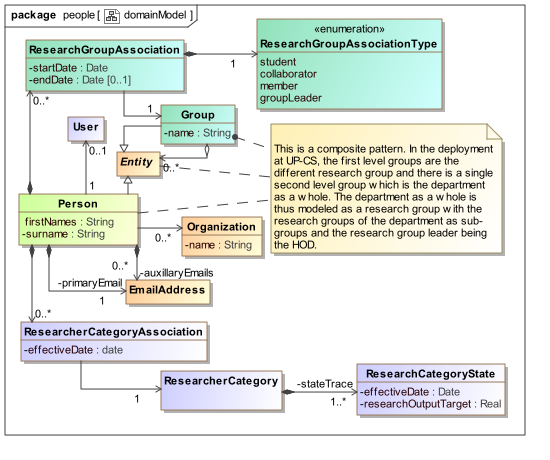
\includegraphics[width=0.8\textwidth,height=0.4\textheight,keepaspectratio=true]{domainModel}
\end{center}
\caption{ \label{fig:users_domainModel} Domain model of users}
\end{figure}

Each user has the following detail associated with his account
\begin{itemize}

\item User name - used as userId
\item Password
\item Title
\item Initials
\item First name
\item Surname
\item Cell number
\item Email address
\end{itemize}

A user is one of two kinds
\begin{itemize}
\item  Admin - indicated with 'A' in the status field.
\item User - indicated with 'U' in the status field.
\end{itemize}

Each user can have multiple associations with teams (See the teams module in Section~\ref{teams}).  

For team allocation purposes, users may be associated with multiple attributes which can be updated using import facilities (see the import and export module in Section~\ref{importExport}) as well as analysis tools (see the analysis module in Section~\ref{analysis})  